\documentclass{standalone}

\usepackage{tikz}
\usetikzlibrary{patterns,arrows,calc,decorations.pathmorphing,backgrounds, positioning,fit,petri,decorations.fractals,trees}
\usepackage{amsfonts}

\newcommand{\complement}{\mathsf{C}}
\begin{document}
	
	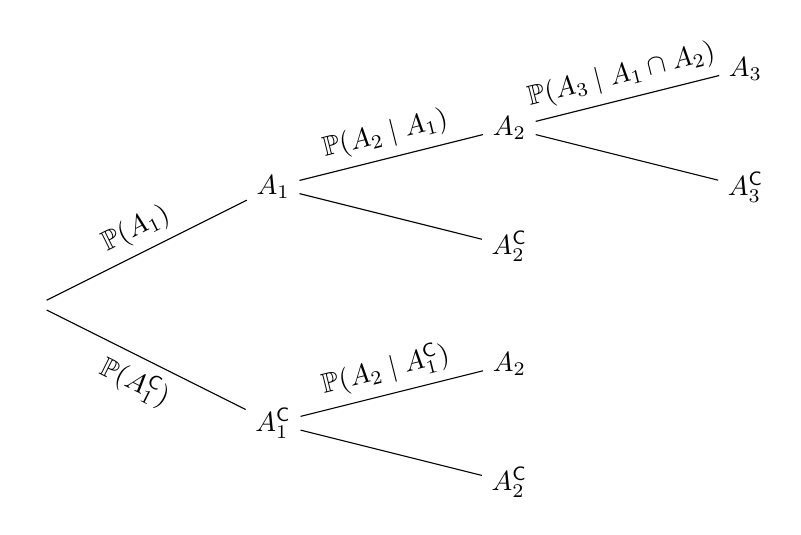
\begin{tikzpicture}[level distance=3cm,
		level 1/.style={sibling distance=3cm},
		level 2/.style={sibling distance=1.5cm},
		grow=right, sloped]
		\node {}
		child {node {$A_1^\complement$}
			child {node {$A_2^\complement$}}
			child {node {$A_2$} edge from parent node[above]  {$\mathbb{P}(A_2\mid A_1^\complement)$}}
			edge from parent
			node[below]  {$\mathbb{P}(A_1^\complement)$}
		}
		child {node {$A_1$}
			child {node {$A_2^\complement$}}
			child {node {$A_2$}
				child {node {$A_3^\complement$}}
				child {node {$A_3$} edge from parent node[above]  {$\mathbb{P}(A_3\mid A_1\cap A_2)$}}
				edge from parent
				node[above]  {$\mathbb{P}(A_2\mid A_1)$}}
			edge from parent
			node[above]  {$\mathbb{P}(A_1)$}
		};
	\end{tikzpicture}

\end{document}}